三组验证结果见表\ref{tab:validation}，均由重复惩罚1.1获得最高ROUGE-L，因此采用该设置进入测试。

\begin{table}[H]
\centering\small
\caption{解码方法比较}\label{tab:validation}
\begin{tabularx}{\linewidth}{Y r r r}
\toprule 模型与新闻输入 & 贪心 & 惩罚1.1 & 禁重复3-gram \\ \midrule
原微调权重，正文 & 27.88 & 28.03 & 27.96 \\
原微调权重，导语加正文 & 29.84 & 30.57 & 30.04 \\
重新微调权重，导语加正文 & 35.21 & 35.63 & 35.14 \\
\bottomrule
\end{tabularx}
\end{table}

\begin{table}[H]
\centering\small
\caption{输入与微调改进结果}\label{tab:refinement}
\begin{tabularx}{\linewidth}{Y l r r r}
\toprule 模型 & 新闻输入 & ROUGE-1 & ROUGE-2 & ROUGE-L \\ \midrule
原微调权重 & 正文 & 31.72 & 18.64 & 29.37 \\
原微调权重 & 导语加正文 & 34.47 & 20.70 & 31.80 \\
重新微调权重 & 导语加正文 & 38.77 & 24.44 & 35.86 \\
首句抽取 & 导语加正文 & 33.34 & 20.24 & 29.41 \\
\bottomrule
\end{tabularx}
\end{table}

表\ref{tab:refinement}中，原权重使用正文并调整解码后，ROUGE-L为29.37，比初始贪心结果高0.60个分值点。加入导语后达到31.80，再提高2.43个分值点。在相同输入和解码下，重新微调达到35.86，相对原权重提高4.06个分值点，相对同输入抽取基线提高6.45个分值点。

总分变化包含解码、输入信息和重新微调三项因素，各项增量依赖当前条件。新增微调的最佳验证交叉熵为3.6074，训练迭代用时9.1分钟。

\begin{figure}[H]

\centering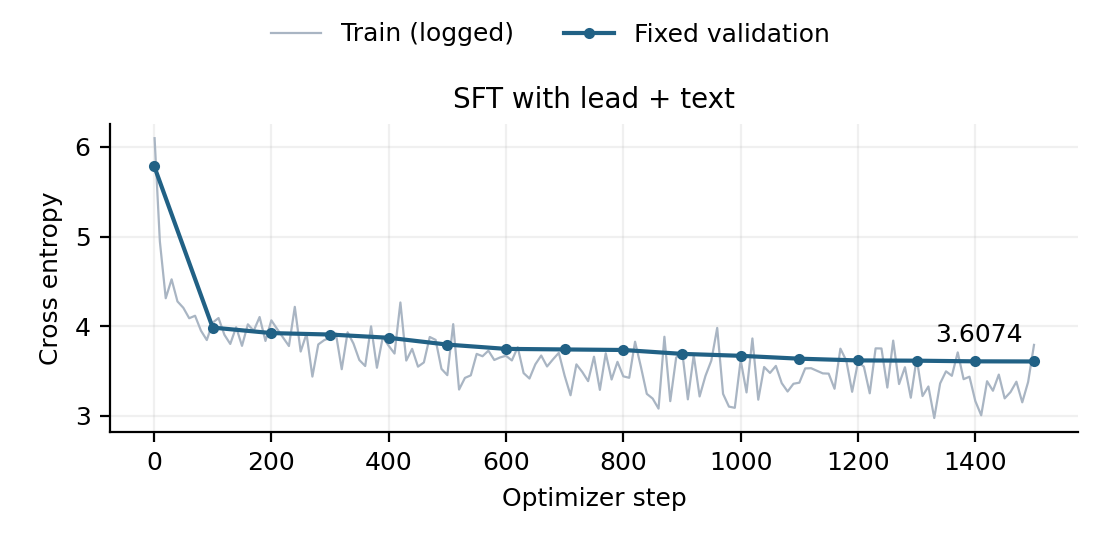
\includegraphics[width=0.82\linewidth]{generated/refinement_curve.png}

\caption{改进微调损失曲线}\label{fig:refinement}

\end{figure}
